\documentclass[border=10pt]{standalone}
\usepackage{tikz,amsmath}
\usetikzlibrary{arrows.meta}

% ========== 配色：绿->蓝->橙->紫->红 ==========
\definecolor{inFill}{RGB}{183,224,177}
\definecolor{inLine}{RGB}{32,102,32}
\definecolor{blFill}{RGB}{214,228,250}
\definecolor{blLine}{RGB}{60,90,170}
\definecolor{orFill}{RGB}{250,224,180}
\definecolor{orLine}{RGB}{190,110,20}
\definecolor{hidFill}{RGB}{199,203,243}
\definecolor{hidLine}{RGB}{52,58,143}
\definecolor{outFill}{RGB}{243,199,199}
\definecolor{outLine}{RGB}{143,52,52}
\definecolor{opFill}{RGB}{250,250,250}
\definecolor{opLine}{RGB}{70,70,70}

\begin{document}
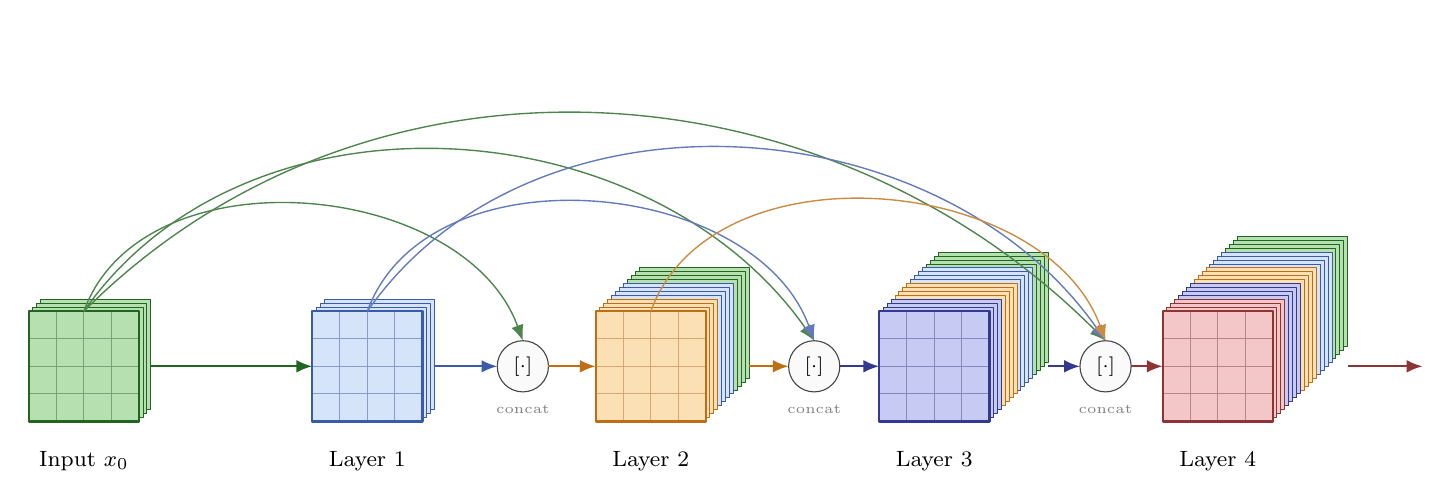
\begin{tikzpicture}[
    font=\small, line join=round,
    every node/.style={inner sep=0pt, outer sep=0pt, align=center},
    >={Latex[length=2mm, width=1.6mm]},
    arr/.style={->, line width=.7pt, rounded corners=3pt},
    dense/.style={->, line width=.5pt},
    add/.style={circle, draw=opLine, fill=opFill, minimum size=.65cm}
  ]

  % ========== 通道增长堆叠宏：l<=1 只 4 片自家；l>=2 = 4 新片 + 全部前驱片 ==========
  \newcommand{\growstack}[3]{%
    \pgfmathtruncatemacro{\Nsh}{ifthenelse(#3<=1, 3, 4+4*#3-1)}
    \foreach \sht in {\Nsh,...,0}{%
      \pgfmathtruncatemacro{\ci}{#3-int(\sht/4)}
      \ifcase\ci \def\cc{in}\or\def\cc{bl}\or\def\cc{or}\or\def\cc{hid}\or\def\cc{out}\fi
      \ifnum\sht=0
        \fill[\cc Fill] (#1,#2) rectangle ++(1.4,1.4);
        \draw[step=.35, \cc Line!60, line width=.4pt, shift={(#1,#2)}] (0,0) grid (1.4,1.4);
        \draw[\cc Line, thick] (#1,#2) rectangle ++(1.4,1.4);
      \else
        \fill[\cc Fill, draw=\cc Line, line width=.3pt]
              ({#1+0.05*\sht},{#2+0.05*\sht}) rectangle ++(1.4,1.4);
      \fi
    }%
  }

  % ================= 五堆叠：4 / 4 / 12 / 16 / 20 片 =================
  \growstack{-7.9}{-0.7}{0}
  \growstack{-4.3}{-0.7}{1}
  \growstack{-0.7}{-0.7}{2}
  \growstack{2.9}{-0.7}{3}
  \growstack{6.5}{-0.7}{4}

  \node[font=\footnotesize] at (-7.2,-1.2) {Input $x_0$};
  \node[font=\footnotesize] at (-3.6,-1.2) {Layer 1};
  \node[font=\footnotesize] at (0,-1.2)    {Layer 2};
  \node[font=\footnotesize] at (3.6,-1.2)  {Layer 3};
  \node[font=\footnotesize] at (7.2,-1.2)  {Layer 4};

  % ================= 主链（★ gap0 无加号，直进 layer1；圆圈=$[\cdot]$=concat） =================
  \draw[arr, inLine] (-6.35,0) -- (-4.3,0);
  % ---- gap 1：concat2 ----
  \draw[arr, blLine] (-2.75,0) -- (-1.95,0);
  \node[add, font=\scriptsize] (p2) at (-1.625,0) {$[\cdot]$};
  \node[font=\tiny, text=gray] at (-1.625,-0.55) {concat};
  \draw[arr, orLine] (-1.3,0) -- (-0.7,0);
  % ---- gap 2：concat3 ----
  \draw[arr, orLine] (1.25,0) -- (1.75,0);
  \node[add, font=\scriptsize] (p3) at (2.075,0) {$[\cdot]$};
  \node[font=\tiny, text=gray] at (2.075,-0.55) {concat};
  \draw[arr, hidLine] (2.4,0) -- (2.9,0);
  % ---- gap 3：concat4 ----
  \draw[arr, hidLine] (5.05,0) -- (5.45,0);
  \node[add, font=\scriptsize] (p4) at (5.775,0) {$[\cdot]$};
  \node[font=\tiny, text=gray] at (5.775,-0.55) {concat};
  \draw[arr, outLine] (6.1,0) -- (6.5,0);
  % ---- 输出 ----
  \draw[arr, outLine] (8.85,0) -- (9.8,0);

  % ================= 密集连接：弧线指 concat 圆顶 =================
  \draw[dense, inLine!80] (-7.2,0.7) to[out=70,in=110] (-1.625,0.325);
  \draw[dense, inLine!80] (-7.2,0.7) to[out=55,in=125] (2.075,0.325);
  \draw[dense, inLine!80] (-7.2,0.7) to[out=45,in=135] (5.775,0.325);
  \draw[dense, blLine!80] (-3.6,0.7) to[out=70,in=110] (2.075,0.325);
  \draw[dense, blLine!80] (-3.6,0.7) to[out=55,in=125] (5.775,0.325);
  \draw[dense, orLine!80] (0,0.7)    to[out=70,in=110] (5.775,0.325);

\end{tikzpicture}
\end{document}